\documentclass[a4paper]{article}

\usepackage[utf8]{inputenc}
\usepackage[english]{babel}

\usepackage{hyperref}
\hypersetup{
    colorlinks=true,
    linkcolor=blue,
    filecolor=magenta,
    urlcolor=cyan,
    citecolor=blue,
    pdftitle={OctaSpace White Paper}
}
\usepackage{graphicx}
\usepackage[parfill]{parskip}
\usepackage{minted}

\graphicspath{ {./img/} }
\usepackage{geometry}
\geometry{
    a4paper,
    total={170mm,257mm},
    left=20mm,
    top=20mm,
}

\begin{document}

\title{OctaSpace White Paper}

\author{OctaSpace Team}

\maketitle

\tableofcontents
\newpage

\begin{abstract}
    OctaSpace is a decentralized cloud computing platform built on blockchain technology.

    It allows individuals and businesses to rent out their unused computing resources in exchange for cryptocurrency payments,
    creating a more cost-effective and sustainable alternative to traditional cloud computing services.

    OctaSpace's unique reward system incentivizes node owners to provide reliable services and maintain the network, while also providing benefits to OCTA coin holders.
    The platform's staking mechanism allows coin holders to earn additional rewards by locking their coins and participating in network validation.

    OctaSpace aims to disrupt the cloud computing industry by providing a secure, transparent, and decentralized solution that benefits both users and providers.
\end{abstract}
\newpage

\section{Introduction}
The backbone of the internet infrastructure is controlled by cloud compute providers that process and store essentially the entire world's data.

With a handful of providers gaining more share each year, the cost of compute will only continue to rise, reducing the number of services that can operate.

To address this, OctaSpace takes a distinct approach by utilizing spare unused compute across the globe to build a scalable distributed compute system that presents itself to users as a unified entity.

With centralization, the need for redundancies also spreads, which increases costs and resources.
These weaknesses can be avoided by utilizing spare unused compute across the globe.

It's essential to have the system with unified interfaces and coherent behavior, providing a single entry point for the end-users' interactions similar to how cloud providers operate today.

With OctaSpace, you can harness the power of CPU, GPU, storage, and traffic resources from Octa nodes across the world to tackle compute-heavy tasks.

By utilizing your spare hardware, it's possible to generate income by acting as a host and renting out your CPU/GPU or traffic.

The hardware required for this can range from basic, low-performance devices or inexpensive VPS to advanced mining rigs and carrier-grade servers located within data centers.

OctaSpace's features and goals:

\begin{itemize}
    \item Utilize a powerful of Hybrid 51\% attack proof blockchain to increase transparency.
    \item Provide easy-to-use interface for describing nodes and executing tasks and marketplace for renting computer focusing on GPU instances
    \item Provide infrastructure to deploy applications and databases mostly close to end-users
    \item Implement a VPN marketplace using popular VPN technologies
    \item Implement distributed data storage and use it as a backbone for CDN service
    \item Increase OctaSpace accessibility globally
\end{itemize}

OctaSpace's focus:

\begin{itemize}
    \item Machine Learning
    \item CGI rendering
    \item Digital image processing
    \item Scientific modeling
    \item Data storing and distributing
    \item VPN technologies
    \item Other tasks/fields which require massive computation power to get be solved
\end{itemize}

\newpage
\section{Architecture}

The following picture shows the core components and interfaces

\begin{figure}[h]
    \centering
    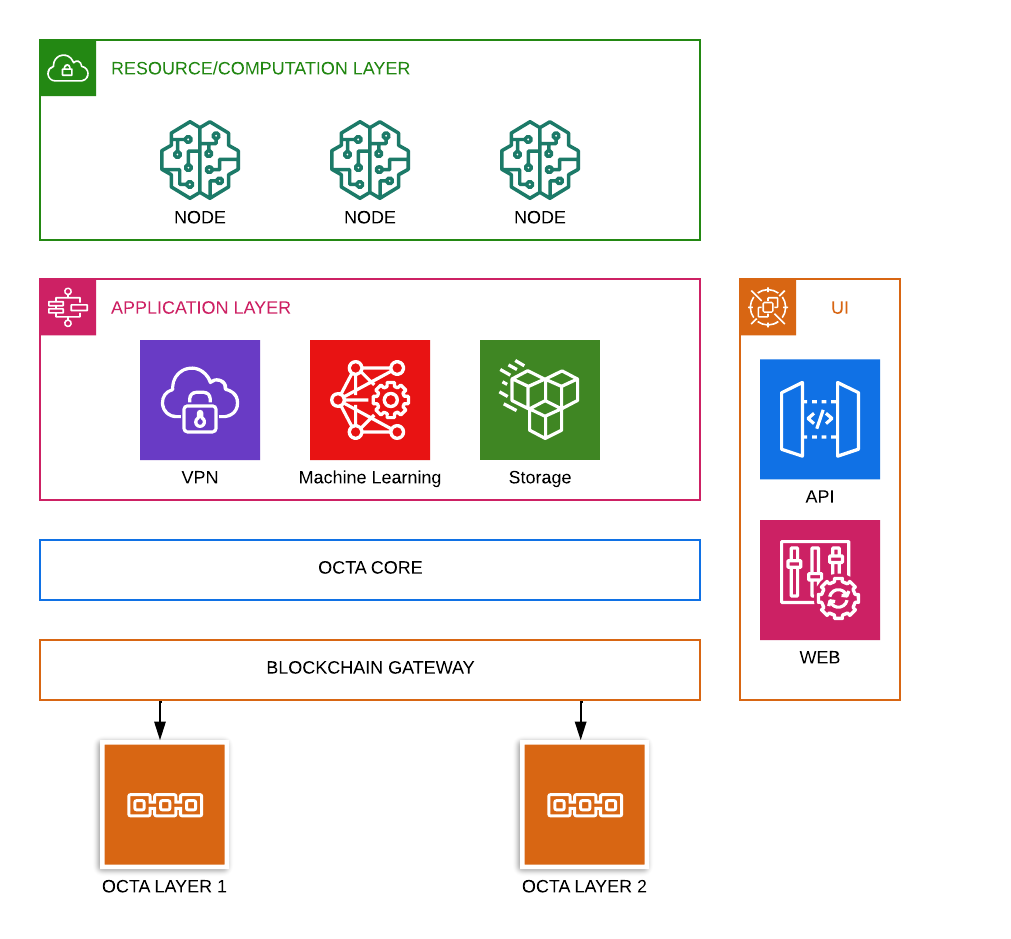
\includegraphics[width=\textwidth]{octa-arch}
    \caption{High Level Architecture}
\end{figure}

\subsection{Blockchain}
Octa Space utilizes a Layer 1 PoW blockchain that is secured using the pirl 51\% guard technique. This security protocol provides protection against attacks on the network, making it a secure platform for users to transact on.

In addition to the Layer 1 PoW blockchain, Octa Space also employs a Layer 2 PoA blockchain that is used to speed up transactions for billing operations. This blockchain is based on validators and is not used to secure the Layer 1 PoW blockchain. By utilizing this Layer 2 PoA blockchain, Octa Space is able to process a large number of transactions quickly and efficiently for billing operations such as charging users for the services they have used.

Overall, Octa Space's use of the pirl 51\% guard and Layer 2 PoA blockchain demonstrate its commitment to security and efficiency. By employing these techniques, Octa Space is able to provide a secure and stable platform for its users while also maintaining fast and efficient transactions for billing operations.

\newpage

\subsection{Layer 1 network}

\textbf{OCTA Layer 1} is PoW\cite{pow} blockchain network is used for the frontend user financial operations using the native coin OCTA.

Network based on go-ethereum\cite{go-ethereum} codebase with the following specification:

\begin{itemize}
    \item Block time is 15 seconds
    \item Total supply is unlimited\footnote{Total supply will be reviewed after Mahasim fork}
    \item Block reward and halving implemented according to \hyperref[sec:mp]{Monenary policy}
    \item PirlGuard is used as protection mechanism from 51\% attack
    \item Transaction fee is 21 Gwei
\end{itemize}

Fair start of the network without premine and with genesis difficulty in 100Gh to prevent instant reward.

\subsection{Layer 2 network}

This is a side chain for Layer 1 network, implemented as PoA\cite{poa} network with a set of validators.

Used for handling internal transactions for the node services its lightning-fast performance and its seamlessly handling of high-frequency, high-usage operations,
resulting in reduced operational costs, speedy transactions and a massive boost in charging operations throughput.

\subsection{Blockchain gateways}

These gateways provides unified API for \textbf{OCTA CORE} layer to give it ability work with both blockchain networks.

This API is private and not accessible outside.

\subsection{OCTA CORE and Application Layer}
The engine of our system, the compute rental manager, seamlessly handles all requests for compute rentals and communicates with the nodes and user applications to make it effortless for users to access and use the resources of connected nodes.

This layer is designed to be user-friendly, so even those without technical expertise can take advantage of the available resources with ease.

Its the core engine of our system, it's responsible for the following operations:

\begin{itemize}
    \item Communicates, monitoring and low level interaction with nodes
    \item Handle requests for computing resources
    \item Provide interface for creating services on a top of resources provided by nodes
    \item Services usage charging and billing operations
    \item Provide API for automation or integration with third party systems
    \item Fraud control
    \item Statistic and telemetry of system usage
\end{itemize}

\subsection{Resource Layer}
While the Octa Chain is very capable at processing large amounts of transactions the real aim of the project is to provide real world applications and to bridge the gap of computational owners and computational users. To accomplish this we’ve built Octa nodes

This layer consist of hardware(nodes) connected to the OctaSpace cloud.

Nodes are the foundation of our compute and services marketplace, providing the necessary computational power to meet the demands of tasks.

These computers are equipped with a blend of CPUs, GPUs, memory, and disk space that allows them to handle distributed workloads with ease.

The nodes are connected to the OctaSpace, which enables them to seamlessly work together to deliver optimal performance and efficiency.

The tasks and services may vary, well equipped machines with powerful GPU may performs AI/ML tasks,
common machines may acts as VPN gateway, provide disk storage for services like file sharing or host applications deployed by users.

\subsection{API and UI}

To work with system the following interfaces available:

\begin{itemize}
    \item Web applicaton with user-friendly interface: \url{https://cube.octa.space}
    \item RESTful API
    \item \textbf{octactl} command-line utility that provide user friendly interface to RESTful API
\end{itemize}

\newpage
\section{Nodes}

In the nutshell node is a Linux machine with special software installed.

This software is called \textbf{ORC}, using it \textbf{OCTA CORE} is able to establish secure communication channel to the node.

Communication between \textbf{OCTA CORE} and \textbf{ORC} is doing in RPC\cite{rpc} like manner.

Secure channel is implemented using HTTPS\cite{https} protocol with validating each request using security token.

\begin{figure}[H]
    \centering
    
\includegraphics[scale=0.5]{core-orc-channel}
    \caption{Secure communication channel}
\end{figure}

\textbf{ORC} is responsible for the following activities:

\begin{itemize}
    \item Detect installed hardware: CPU, GPUs, RAM, volume of disk storage
    \item Collect metrics about hardware usage, like free/used disk/ram space, CPU and GPU load, temperature and fans speed
    \item Manage Docker\cite{docker} containers and Firecracker\cite{firecracker} microVMs
\end{itemize}

There are two types of nodes: \textbf{blockchain} and \textbf{service}

The first one is responsible for support of OCTA Layer 1 blockchain by running network node software.
As a result such nodes making network more stable, distributed, more latency fair and speed up the synchronization.

Service node provides resources we used to implement services for the end users.

\subsection{Hardware and software requirements}

To cover a wide range of supported hardware, node software can be installed on any machine with x86\_64\cite{x86_64} or ARM\cite{arm} architecture.

In order to run the node, the hardware must meet the minimum system requirements, which are as follows: 1 CPU, 1 Gb of RAM, and 10Gb of free disk space.

However, the requirements for hardware may vary depending on the intended purpose of the node. For instance, a node that provides only VPN services may only need to meet the minimum requirements. Conversely, nodes that are designed to perform AI/ML tasks will require powerful GPUs connected with a high bandwidth PCIe interface, as well as ample disk storage.

It's worth noting that both NVIDIA and AMD GPUs are supported by the system.

To determine the performance of a node, the following measurements are taken:

\begin{itemize}
    \item Network upload/download speed
    \item Disk write speed
    \item GPU performance using AI benchmark (only for NVIDIA)
\end{itemize}

These performance metrics help users to choose the hardware they need for their tasks.

The node software can be installed on any Linux distribution; however, we primarily focus on Ubuntu LTS or Debian as the recommended operating systems.

Support for Windows in development.

\subsection{Security}

To eliminate possible security risks for users running the software \textbf{ORC} on their machines, we follow a set of rules and guidelines, which include: 

\begin{itemize}
    \item \textbf{ORC} is open sourced, this may possible to make audit by other people that software does not have malicious code
    \item Keep code base of \textbf{ORC} is small as possible for ease auditing
    \item Node software run under non privilaged user and don't have any permissions which not need for operation
    \item Regular software updates to ensure that the latest security patches are applied. Along with comprehensive testing of software to detect and address any potential security issues.
\end{itemize}

\subsection{Verification}

Ensuring that node infrastructure operates smoothly and reliably is crucial for providing high-quality services to end-users.

Each new node that joins the cloud must be verified and confirmed to meet the necessary requirements and provide services.

Periodically, we conduct re-verification checks on verified nodes. Therefore, it's crucial to monitor the status of your nodes to avoid having them changed to an unverified status.

The checks performed to ensure that the node is properly configured may include but are not limited to:

\begin{itemize}
    \item Meet minimum hardware requirements
    \item System clock is synchronized
    \item All necessary network ports are open
    \item GPU driver is correctly installed
\end{itemize}

The list of checks will be expanding in the future to ensure even greater accuracy and reliability.

The following restrictions are applied for the unverified nodes:

\begin{itemize}
    \item Nodes can't provide services
    \item Nodes can't participate in \hyperref[sec:staking]{staking}
\end{itemize}

\newpage
\section{Services}

Services are what we build and what the project offers to end users.

These are things that can be used every day to solve problems from different areas, from complex calculations to simple file sharing between friends.

Below are some of the services that we have implemented or plan to implement in the near future.

In our opinion, these services that may be of interest to users and will find applications for every day.

\subsection{GPU marketplace}

This service provide ability to rent or rent out GPUs power.

This power may used to solve tasks in AI/ML, CGI rendering or any other fields where powerful GPUs is necessary.

Because we support both NVIDIA and AMD this increase the spectrum of tasks be solved.

Access to the rented instances is provided via SSH\cite{SSH} protocol.

Also it's possible to use Jupyter\cite{jupyter} and LiveBook\cite{livebook} systems for interactive access.

The rented GPU instances can be combined into a cluster, which makes it possible to run and develop distributed programs,
for example distributed training of ML models using TensorFlow\cite{tensorflow} or PyTorch\cite{pytorch}.

\subsection{VPN}

OCTA VPN\cite{VPN} offers a variety of key benefits to its users.
One of the main advantages is its ease of setup, which is made possible by utilizing non-modified and open-source software that is compatible with a wide range of platforms.

Additionally, users have the flexibility to choose from a variety of VPN technologies to suit their needs.
There are also no limitations on the number of devices that can be connected simultaneously.

To add to that, the billing model is pay-as-you-go, which means you are billed only for the amount of data you use.
This gives you complete control over your usage and costs.

Service don’t any logging of the user traffic or DNS requests.

VPN access is implemented using the following technologies:

\begin{itemize}
    \item WireGuard
    \item ShadowSocks
    \item OpenVPN
\end{itemize}

In the future more VPN types will be added, including some to bypass China's golden shield (Great Firewall of China).
\subsection{Remote Video Gaming}

Many have tried and failed with Stedia recently falling. All these services essentially rely on massive centralized server farms which inherently introduces huge latency issues resulting in bad gaming experience if your not located with 100km of the facility.

But with OctaSpace and enough nodes it may finally be possible for a remote gaming service to be widly used utilizing nodes across the globe allowing gamers to use share unused hardware. By connecting to say your neighbours unused pc would solve the major problem of latency in remote gaming services.

\subsection{HashCache}

HashCache is a Password Recovery service for performing password cracking operations on a large scale. It utilizes multiple nodes working together in a coordinated manner to speed up the cracking process. This is achieved by dividing the cracking workload among the nodes, allowing them to work in parallel on different parts of the task.

The system is designed to be highly configurable and can be optimized for different types of cracking operations, such as dictionary attacks, brute force attacks, and others.

\subsection{Distributed Rendering}

Another service example would be a distributed handbrake video encoding network. To allow content creators or studios to quickly render out massive edits economically.

\subsection{Instant File Sharing}

This service provide a easy way to upload a file, share a short link, and after it is downloaded, the file is completely deleted.

Key benefits:

\begin{itemize}
    \item All files are encrypted
    \item It's possible to set expiration (Time To Live), after such period file will be deleted
    \item Simple RESTful API
\end{itemize}

\newpage
\section{Monetary Policy}
\label{sec:mp}

Due to unlimited emission to prevent fast growing inflation the following monetary policy is implemented:

\begin{table}[h!]
\centering
\begin{tabular}{||c c c c c c||}
    \hline
        Era & Start block & Total & Miner & Staking & Dev \\ [0.5ex]

        \hline\hline
        Octa & 1 & 8 & 6.5 & 0 & 1.5 \\
        Arcturus & 650000 & 8 & 5 & 1.5 & 1.5 \\
        Oldenburg & 1000000 & 7.5 & 4 & 2 & 1.5 \\
        Zagami & 1500000 & 7 & 3.5 & 2.5 & 1 \\
        Springwater & 2000000 & 6.5 & 3 & 3 & 0.5 \\
        Polaris & 2500000 & 6 & 2.8 & 2.8 & 0.4 \\
        Mahasim & 3000000 & 5 & 2.3 & 2.3 & 0.4 \\ [1ex]
    \hline

\end{tabular}
\caption{Reward distribution according to era}
\label{table:1}
\end{table}

This policy should decrease inflation by changing amount of block reward dependents of era.


\begin{table}[h!]
\centering
\begin{tabular}{||c c c c c||}
    \hline
        Era & Start date & End date & Total coins & Duration \\ [0.5ex]

        \hline\hline
        Octa & Jun 19 2022 & Oct 09 2022 & 5\_200\_000 & $\approx$112 days \\
        Arcturus & Oct 09 2022 & Dec 08 2022 & 2\_800\_000 & $\approx$60 days \\
        Oldenburg & Dec 08 2022 & Mar 04 2023 & 3\_750\_000 & $\approx$86 days \\
        Zagami & Mar 04 2023 & May 09 2023 &  3\_500\_000 & $\approx$86 days \\
        Springwater & May 09 2023 & Aug 23 2023 & 3\_250\_000 & $\approx$86 days \\
        Polaris & Aug 23 2023& Nov 17 2023 & 3\_000\_000, & $\approx$86 days \\
        Mahasim & Nov 17 2023 & $\infty$ & 2\_500\_000 & $\infty$ \\ [1ex]
    \hline

\end{tabular}
\caption{Approximate calculation of era timeline and reward distribution}
\label{table:1}
\end{table}

Total amount of coins mined before Mahasim era is $\approx$18\_350\_000

\newpage
\section{Staking}
\label{sec:staking}

To incentive interest of holding the staking mechanism is introduced.

Using it people who locked some amount of coins and run node is rewarded.

There are requirements which need met to activate staking:

\begin{itemize}
    \item Collateral - 100\_000 OCTA
    \item Node reliability for the last 30 days $\ge$ 75\%
    \item Node must be verified
\end{itemize}

To start staking it's necessary to have the address wallet with enough balance and link it to existing node.
Reward will be come to the wallet provided.

If system detect balance less than collateral staking will be disabled for such wallet-node pair for
several rounds.

\subsection{Reward distribution scheme}

The billing period is 1 week (every 7 days).

Let's assume that block time is always 15 seconds then the following amount of blocks would be mined:

\begin{itemize}
    \item 1 minute - 4
    \item 1 hour - 240
    \item 1 day - 5760
    \item 7 days - 40320
    \item 30 days - 172800
\end{itemize}

In this calculation we will use reward amount for Arcturus and Oldenburg eras where 1.5 OCTA from each block going to staking fund.

The total amount of coins mined for 1 week would be 60480 OCTA.

Let’s assume we have 10 nodes up and running, then the 60480 OCTA would be distributed across they in the following proportion:

\begin{itemize}
    \item 60\% (base reward) - 36240 OCTA, 3624 for each node
    \item 20\% (gpu reward) - 12080 OCTA, 1208 for each node which provide renting service with GPU
    \item 10\% (vpn reward) - 6040 OCTA, 604 for each node which provide VPN service
    \item 10\% (rent reward) - 6040 OCTA, 604 for each node which provide renting service
\end{itemize}

In case of no nodes for which needs to distribute 40\% (except base reward) the coins will be left in staking fund for the next round.

Most profitable variant is to have node with GPU and which provides both services.
Such node will be rewarded by 6040 OCTA per week and also additional payments for services usage.

Due to the current scheme, we can calculate minimal monthly ROI in the following way:

\[
    ROI = \frac{MonthReward / Collateral * 100}{N} = \frac{M}{100} * 60
\]

Where \textbf{MonthReward} is 172800 blocks multiply by staking reward according to current era.

\textbf{N} is amount of nodes participated in staking, for example 10.

Therefore the minimal ROI for Arcturus and Oldenburg eras will be:

\[
    ROI = \frac{172800 / 100000 * 100}{10} = \frac{17.28}{100} * 60 = 10.36\%
\]


\bibliography{paper}
\bibliographystyle{plain}

\end{document}
